
\section{Avalanche involving a dry area}

An avalanche problem involving a dry area is solved using shallow water approach. This problem is very similar to the dry dam break, but it is on a sloping topography. The debris could be snow, sand, or even rock. The simulation should show a rarefaction and wetting process, just like the dry dam break problem. The analytical solution of this problem was derived by Mungkasi and Roberts~\cite{MR2011DA}. This shallow water approach to solve debris avalanche problems was also implemented by a number of researchers, such as Mangeney et al.~\cite{MHR2000} and Naaim et al.~\cite{NVC1997}. 

The initial condition is
\begin{equation} \label{eq:dap_init}
u(x,0)=0, ~~v(x,y)=0, ~~\textrm{and}~~
h(x,0) = \left\{ \begin{array}{ll}
h_1 & \textrm{if $x < 0$}\\
0 & \textrm{if $x > 0$}\\
\end{array} \right.
\end{equation}
where $h_1>0$. The topography is a flat bed with positive slope.

The analytical solution~\cite{MR2011DA} at time $t>0$ is
\begin{equation} 
h(x) = \left\{ \begin{array}{ll}
0 & \textrm{if $x \leq -2 c_0 t + \frac12 mt^2$}\\
h_R=\frac{1}{9g} \left( \frac{x}{t} + 2c_0 - \frac12 mt \right)^2 & \textrm{if $-2 c_0 t + \frac12 mt^2 \leq x \leq c_0 t + \frac12 mt^2$}\\
h_0 & \textrm{if $x \geq c_0 t + \frac12 mt^2$}\\
\end{array} \right.
\end{equation}
which is the free surface and
\begin{equation} 
u(x) = \left\{ \begin{array}{ll}
0 & \textrm{if $x \leq -2 c_0 t + \frac12 mt^2$}\\
u_R=\frac23 \left( \frac{x}{t} - c_0 + mt \right) & \textrm{if $-2 c_0 t + \frac12 mt^2 \leq x \leq c_0 t + \frac12 mt^2$}\\
mt & \textrm{if $x \geq c_0 t + \frac12 mt^2$}\\
\end{array} \right.
\end{equation}
which is the velocity. Here $m=-g\tan{\theta}+F$, where $\tan{\theta}$ is the slope of the topography. Variable $F$ is the Coulomb-type friction given by 
\begin{equation}
F=g \cos^2{\theta} \tan{\delta},
\end{equation}
in which $\tan{\delta}$ is a given value of friction slope such that $\tan{\delta} \leq \tan{\theta}$.


\subsection{Results}

For our test, we consider $h_0=20$ in (\ref{eq:dap_init}).
The following figures show the stage, $x$-momentum, and $x$-velocity at several instants of time. We should see excellent agreement between the analytical and numerical solutions. The wet/dry interface is difficult to resolve and it usually produces large errors, similar to the dry dam break problem.
\begin{figure}[h]
\begin{center}
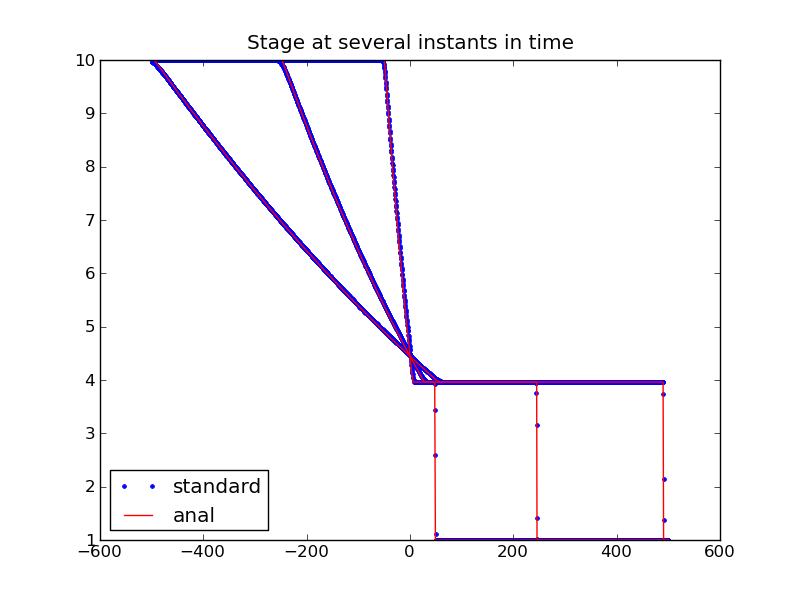
\includegraphics[width=0.9\textwidth]{stage_plot.png}
\end{center}
\caption{Stage results}
\end{figure}


\begin{figure}[h]
\begin{center}
\includegraphics[width=0.9\textwidth]{xmom_plot.png}
\end{center}
\caption{Xmomentum results}
\end{figure}


\begin{figure}[h]
\begin{center}
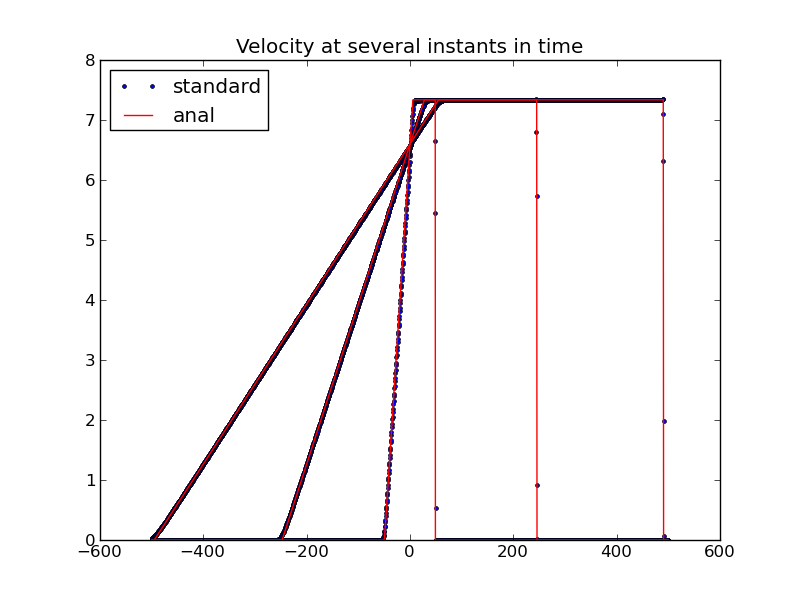
\includegraphics[width=0.9\textwidth]{xvel_plot.png}
\end{center}
\caption{Xvelocity results}
\end{figure}


\endinput
